\documentclass[11pt]{article}
\usepackage[utf8]{inputenc}
\usepackage[T1]{fontenc}
\usepackage{fixltx2e}
\usepackage{graphicx}
\usepackage{longtable}
\usepackage{float}
\usepackage{wrapfig}
\usepackage{rotating}
\usepackage[normalem]{ulem}
\usepackage{amsmath}
\usepackage{textcomp}
\usepackage{marvosym}
\usepackage{wasysym}
\usepackage{amssymb}
\usepackage{capt-of}
\usepackage{hyperref}
\tolerance=1000
\usepackage{minted}
\usepackage{color}
\usepackage{listings}
\usepackage{grffile}
\usepackage[inline]{enumitem}
\usepackage{setspace}
\usepackage{tikz}
\usepackage{subcaption}
\usepackage{xcolor}
\usepackage{fancyvrb}
\hypersetup{
colorlinks,
linkcolor={red!50!black},
citecolor={blue!50!black},
urlcolor={blue!80!black}
}
\usepackage{setspace}%% The linestretch
\singlespacing
\usepackage[format=hang,indention=0cm,singlelinecheck=true,justification=raggedright,labelfont={normalsize,bf},textfont={normalsize}]{caption} %
\usepackage{vmargin}
\setpapersize{A4}
\setmarginsrb{2.5cm}{1cm}% links, oben
{2.5cm}{2cm}% rechts, unten
{12pt}{30pt}% Kopf: Höhe, Abstand
{12pt}{30pt}% Fuß: Höhe, AB
\usepackage{upquote}
%  use straight quotes when printing a command in minted
\AtBeginDocument{%
\def\PYZsq{\textquotesingle}%
}
\definecolor{mintedbackground}{rgb}{0.95,0.95,0.95}
\setlength{\parindent}{0pt}
\setlength{\parskip}{\baselineskip}
\definecolor{mintedbackground}{rgb}{0.95,0.95,0.95}
\definecolor{mintedBg}{rgb}{0.95, 0.95, 0.95}
\definecolor{blockBg}{rgb}{0.6, 0.6, 0.95}

%% define styles for different codes
\newminted{cpp}{linenos, bgcolor=blockBg, fontsize=\footnotesize}
%% then use \begin{cppcode}
\newminted{c}{linenos, bgcolor=mintedBg, fontsize=\footnotesize}
\newminted{perl}{linenos, bgcolor=mintedBg, fontsize=\footnotesize}
\newminted{r}{linenos, bgcolor=mintedBg, fontsize=\footnotesize}


%% I detest indentation in footnotes etc, so try this:
\makeatletter
\renewcommand\@makefntext[1]{\noindent\makebox[0em][r]{\@makefnmark}\footnotesize#1}
\makeatother
%% the makeatletter and makeatother are required to allow me to
%% to change the macro beginning with an @. (though when I call it
%% I don't use the @ ... 

%% this should handle non-breaking space
%% characters.
\DeclareUnicodeCharacter{00A0}{~}

\renewcommand\scriptsize\normalsize

\author{Martin Jakt\thanks{University of Nordland, Norway}}
\date{2015-11-10}
\title{\textbf{Course assignment Overview}}
\hypersetup{
  pdfkeywords={},
  pdfsubject={},
  pdfcreator={}}

\begin{document}

%\maketitle
%\tableofcontents

\section{Overview}
\begin{figure}[ht]
  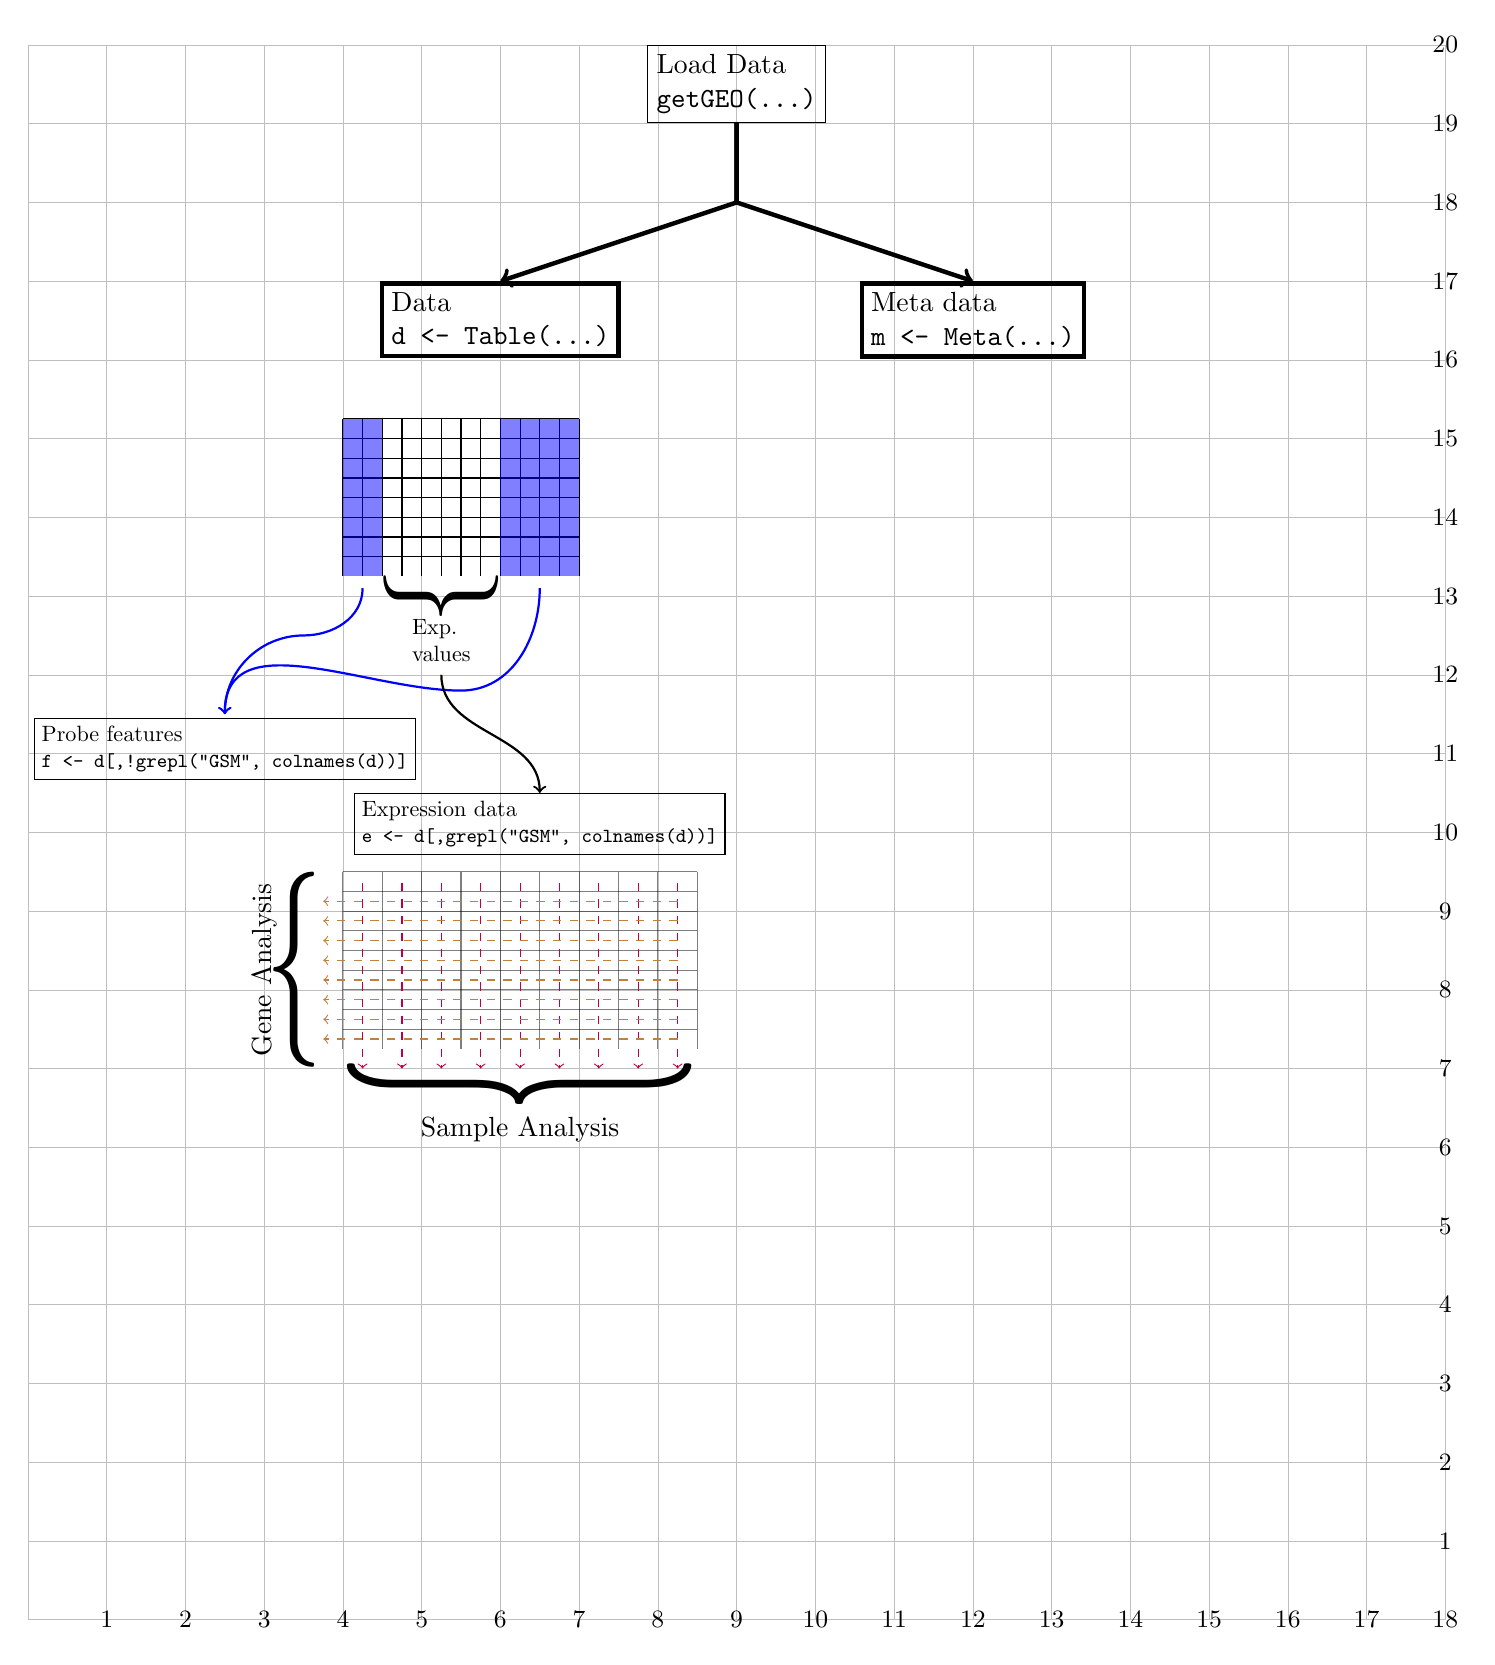
\begin{tikzpicture}{scale=0.5}
    \draw [help lines, opacity=0.5] (0,0) grid (18,20);
    \foreach \x in {1,2,...,18} \node [font=\small] at (\x,0) {\x};
    \foreach \y in {1,2,...,20} \node [font=\small] at (18,\y) {\y};
    \node [below, draw, align=left] (l1) at (9,20) {
      Load Data\\
      \texttt{getGEO(...)} };
    \draw [->, ultra thick] (l1.south) -- (9,18) -- (6,17) node [below, draw, align=left] (t1) 
    {Data\\ \texttt{d <- Table(...)}};
    \draw [->, ultra thick] (l1.south) -- (9,18) -- (12,17) node [below, draw, align=left] (m1)
    {Meta data\\ \texttt{m <- Meta(...)}};
    %% draw a table looking thing
    \foreach \x in {4, 4.25, ..., 7} \draw [-] (\x,15.25) -- (\x,13.25);
    \foreach \y in {15.25, 15, ..., 13.5} \draw [-] (4,\y) -- (7,\y);
    \path [fill=blue, opacity=0.5] (4,13.25) rectangle (4.5, 15.25);
    \path [fill=blue, opacity=0.5] (6,13.25) rectangle (7, 15.25);
    \node [rotate=-90, scale=2] (cb1) at (5.25,13) {\huge\}};
    \node [scale=0.8, below, align=left] at (5.25,12.8) 
       {Exp.\\values};
    \draw [->, thick, blue] (4.25,13.1) to [out=270,in=0] (3.5,12.5)
       to [out=180,in=90] (2.5,11.5);
    \draw [->, thick, blue] (6.5,13.1) to [out=270,in=0] (5.5, 11.8)
       to [out=180,in=90] (2.5,11.5);
    \node [draw, below, align=left, scale=0.8] (f1) at (2.5,11.45) {
      Probe features\\
      \small\texttt{f <- d[,!grepl("GSM", colnames(d))]}};

    \draw [->, thick] (5.25,12) to [out=270,in=90] (6.5,10.5);
    \node [draw, below, align=left, scale=0.8] at (6.5,10.5)
      {Expression data\\
       \small\texttt{e <- d[,grepl("GSM", colnames(d))]}};
 
    \foreach \x in  {4, 4.5, ..., 8.5} \draw [-, opacity=0.5]
      (\x,9.5) -- (\x,7.25);
    \foreach \y in {9.5, 9.25, ..., 7.5} \draw [-,opacity=0.5]
      (4,\y) -- (8.5,\y);

    \foreach \x in  {4.25, 4.75, ..., 8.25} \draw [->, dashed, purple]
      (\x,9.36) -- (\x,7);
    \foreach \y in {9.125, 8.875, ..., 7.375} \draw [->, dashed, brown]
      (8.25,\y) -- (3.75,\y);
    \node [rotate=-90, xscale=2, yscale=6] at (6.25, 6.8) {\huge\}};
    \node [xscale=2, yscale=3.4, left] at (4, 8.25) {\huge\{};
    
    \node [below, align=left] at (6.25, 6.5) {Sample Analysis};
    \node [align=left, rotate=90] at (3,8.25) {Gene Analysis};

  \end{tikzpicture}
  \caption{An overview}
  \label{overview}
\end{figure}

The general overview of the flow of data is shown in Fig. \ref{overview}.

\end{document}